\documentclass{article}

\usepackage{graphicx} % for images
\usepackage{amsmath} % for math
\usepackage{amssymb} % for \mathbb
\usepackage{siunitx} % for \SI, \num
\usepackage{hyperref} % for \url{}

% DO NOT COPY
\graphicspath{{"C:/Users/oscar/Coding Projects/CSULB/CECS 463 SPRING 2021/Homework 2/html/"}}

% This stuff is for figures
\usepackage{float}
\DeclareGraphicsExtensions{.pdf, .png, .jpg}

% coloring of links for PDF format
\hypersetup{
    colorlinks=true,
    urlcolor=blue,
    linkcolor=blue
}

% \c command redefinition (for monospaced font)
\renewcommand{\c}[1]{\texttt{#1}}
% \today command re-definition
% https://tex.stackexchange.com/questions/112932/today-month-as-text
\renewcommand{\today}{\ifnum\number\day<10 0\fi \number\day \space%
\ifcase \month \or January\or February\or March\or April\or May%
\or June\or July\or August\or September\or October\or November\or December\fi\space%
\number \year} 

\begin{document}

\noindent
Rodrigo Becerril Ferreyra\\
Dr. Alireza Mehrnia\\
Homework 2\\
\today

The code used to generate all plots is given at the end
of this document.

\addcontentsline{toc}{section}{P2.2}
\section*{P2.2} Below are the plots generated according to the
instructions in P2.2 of the class textbook.

\begin{figure}[H]
    \centering
    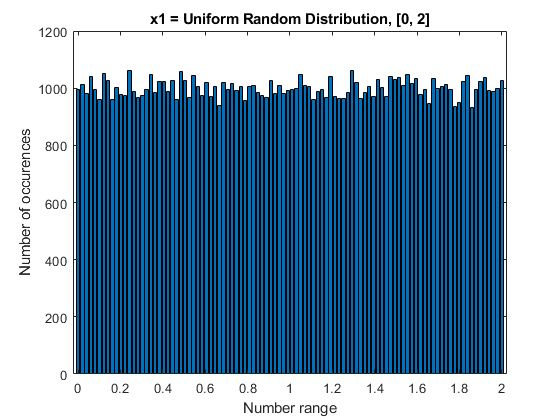
\includegraphics[width=0.9\textwidth]{HW2_01}
    \caption{P2.2.1}
    \label{P2.2.1}
\end{figure}

\begin{figure}[H]
    \centering
    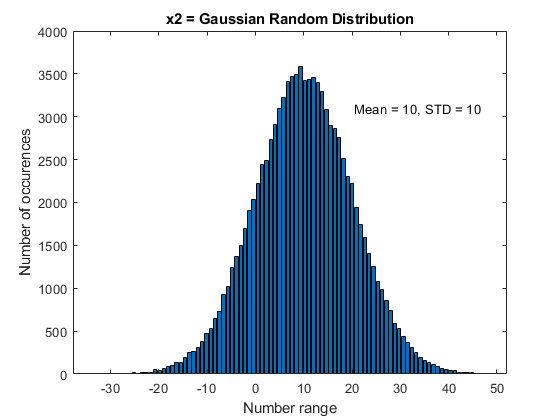
\includegraphics[width=0.9\textwidth]{HW2_02}
    \caption{P2.2.2}
    \label{P2.2.2}
\end{figure}

\begin{figure}[H]
    \centering
    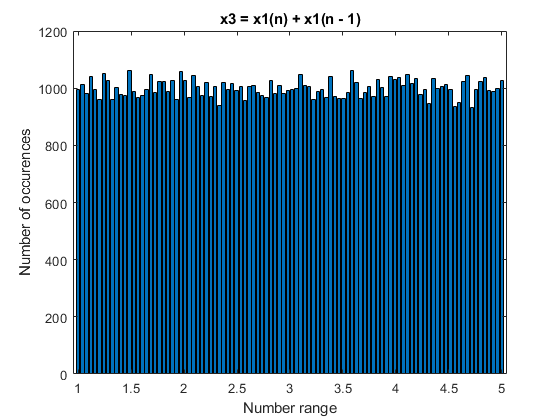
\includegraphics[width=0.9\textwidth]{HW2_03}
    \caption{P2.2.3}
    \label{P2.2.3}
\end{figure}

\begin{figure}[H]
    \centering
    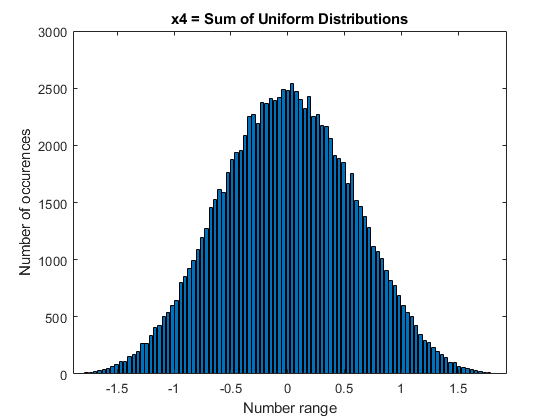
\includegraphics[width=0.9\textwidth]{HW2_04}
    \caption{P2.2.4}
    \label{P2.2.4}
\end{figure}

Figures \ref{P2.2.3} and \ref{P2.2.4} were generated similarly:
They are sums of multiple random variables uniformly
distributed. Figure \ref{P2.2.3} is the sum of the random variable
shown in Figure \ref{P2.2.1} added with an index-shifted
version of itself, while Figure \ref{P2.2.4} is the sum of four
individual random variables uniformly distributed over the range
\([-1/2, 1/2]\). The difference between the two plots is
self-evident: the former resembles a uniform distribution,
while the latter resembles a normal distribution. This is
due to the central limit theorem: informally, as one sums
independent random variables with the same distribution,
the sum of the random variables is itself normally distributed.

\addcontentsline{toc}{section}{P2.3}
\section*{P2.3}
The following are plots generated for sections 2 and 3 of
Problem 2.3.

\begin{figure}[H]
    \centering
    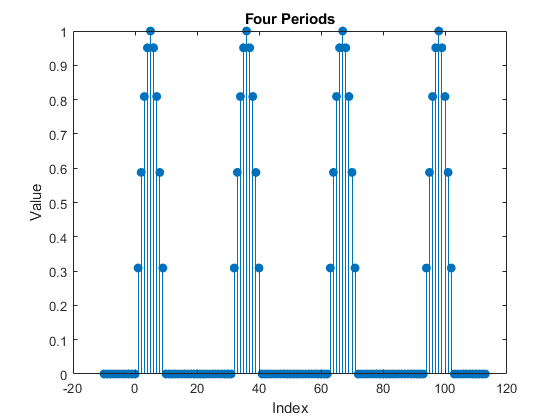
\includegraphics[width=0.9\textwidth]{HW2_06}
    \caption{P2.3.3}
    \label{P2.3.3}
\end{figure}%
\begin{figure}[H]
    \centering
    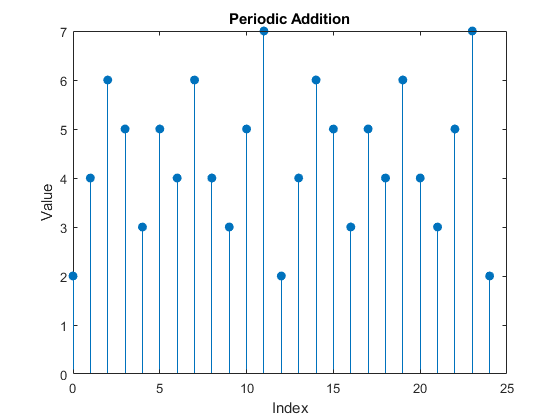
\includegraphics[width=0.9\textwidth]{HW2_07}
    \caption{P2.3.4}
    \label{P2.3.4}
\end{figure}

The period of Figure \ref{P2.3.4} is the number of indexes
between the lowest two points (in this case, when the value is
\num{2}); this means that the period is \num{12}. The value 2
occurs at index 0, 12, and 24. This is
because the periods of the two periodic signals used to create
this plot are 3 and 4 (and \(3 \times 4 = 12\)).

\addcontentsline{toc}{section}{P2.5}
\section*{P2.5}

The following theorem was given:
``The complex exponential sequence \(\exp(j\omega_0n)\)
or the sinusoidal sequence \(\cos(\omega_0n)\) are periodic if
the \emph{normalized} frequency \(f_0 \equiv \omega_0/2\pi\)
is a rational number; that is, \(f_0 = K/N\) such that
\(K, N \in \mathbb{Z}\).''

Note that the following proof
is for \(\cos(\omega_0n)\), but applies to both the real and
imaginary parts of
\(\exp(j\omega_0n)\) as well, due to Euler's formula that states
that \(\operatorname{Re}\left(e^{jx}\right) = \cos(x)\) and
\(\operatorname{Im}\left(e^{jx}\right) = \sin(x)\). In addition,
\( \sin(\pi/2 - x) = \cos(x) \). Therefore, this proof
applies to both cases.

In the continuous case, it is always true that a sinusoid such
as the cosine
function is periodic. However, for the discrete case, the
normalized frequency \(f_0 \equiv \omega_0 / 2\pi\) must be a
rational number.
Remember that a sequence \(x(n)\) is periodic if
\begin{equation} \label{periodic def}
    x[n] = x[n + P] \text{ for all } n,
\end{equation}
where \(P\) is the
fundamental period (textbook, p. 25). In the case of
\(f_0 \equiv K/N\), \(N\) will be the fundamental period
(i.e., \(x(n) = x(n + N)\) for all \(n\)).
For example, if \(f_0 = 3/8\), then \(8\) will be the
fundamental period (\(x(n) = x(n + 8)\) for all \(n\)).%
\footnote{This was discovered numerically by using
the Desmos graphing calculator to graph sinusoids,
available at \url{https://www.desmos.com/calculator}.}
The number 3 is the amount of continuous periods
the sinusoid must go through before a period starts on
an integer index. For example, for the signal
\(x(n) = \cos(0.75\pi n)\), \(x(0) = 1\).
\(x(8/3)\), \(x(2\times 8/3)\), and \(x(3\times 8/3)\) all also
equal \(1\), but \(3\times 8/3 = 8\) is the only index that
is an integer and thus valid for a discrete signal; in the
discrete case, \(x[0] = 1\), and the first sample that will
also equal \(1\) is \(x[8]\); thus, 8 will be the
fundamental period.
If \(f_0\) is not a
rational number, \(N\) is not defined/does not exist. Therefore,
for a discrete signal to be periodic, \(f_0\) must be rational.

The following are plots generated for Problem 2.5. Figure
\ref{P2.5.2} was generated using \(z = \exp(j 0.1 \pi n)\),
and Figure \ref{P2.5.3} was generated using \(x = \cos(0.1n)\).

\begin{figure}[H]
    \centering
    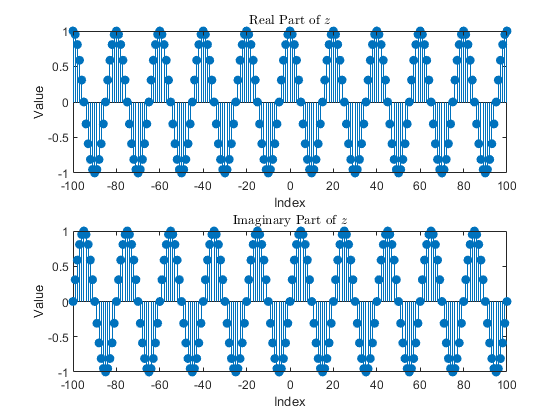
\includegraphics[width=0.9\textwidth]{HW2_08}
    \caption{P2.5.2}
    \label{P2.5.2}
\end{figure}%
\begin{figure}[H]
    \centering
    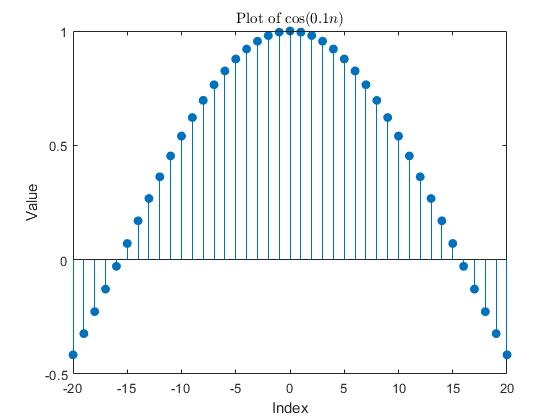
\includegraphics[width=0.9\textwidth]{HW2_09}
    \caption{P2.5.3}
    \label{P2.5.3}
\end{figure}

Both the real and imaginary parts of Figure \ref{P2.5.2} are
indeed periodic. The normalized frequency is
\begin{equation*}
    f_0 = \frac{0.1\pi}{2\pi} = \frac{1}{20}.
\end{equation*} Thus, \(K = 1\) and \(N = 20\), and its fundamental
period is \(N = 20\). This can be seen graphically by noticing
that the value of zero is achieved on the indexes that are
integer multiples of 20 (\(\{20k \mid k \in \mathbb{Z}\}\)).

The sinusoid presented in Figure \ref{P2.5.3} is not periodic.
It certainly looks like it is, but numerically, it does not
satisfy the definition of periodicity
(Equation \eqref{periodic def}). Its normalized frequency is
\begin{equation*}
    f_0 = \frac{0.1}{2\pi} = \frac{1}{20\pi}.
\end{equation*} \(K = 1\) and \(N = 20\pi\), so its fundamental
frequency is \(20\pi\). However, since this is not an integer,
it cannot be used in the practice of discrete signals, where
all indexes are integers. Thus, it is not periodic.

\addcontentsline{toc}{section}{P2.6}
\section*{P2.6}

The following are plots generated for sections 3 and 4 of
Problem 2.6. These graphs were obtained by using the \c{evenodd}
function provided in the textbook (p. 34).

\begin{figure}[H]
    \centering
    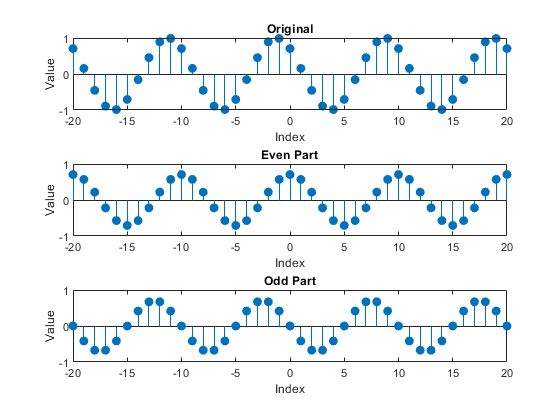
\includegraphics[width=0.9\textwidth]{HW2_11}
    \caption{P2.6.3}
    \label{P2.6.3}
\end{figure}%
\begin{figure}[H]
    \centering
    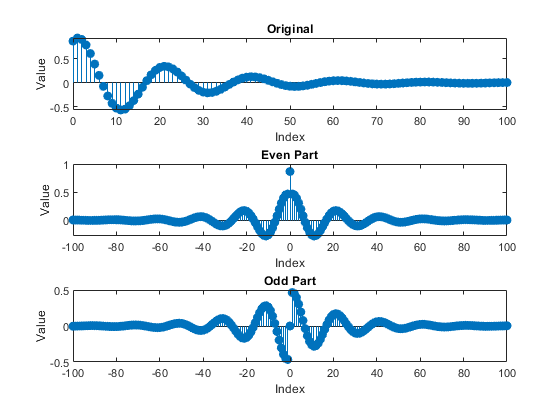
\includegraphics[width=0.9\textwidth]{HW2_12}
    \caption{P2.6.4}
    \label{P2.6.4}
\end{figure}%

\addcontentsline{toc}{section}{P2.10}
\section*{P2.10}

Let \(y(n) = x(n) + \alpha x(n - k)\), where \(x(n)\) is a
signal, and \(\alpha x(n - k)\) is its echo (noise). The
cross-correlation between \(y\) and \(x\) is given by
\begin{equation*}
    r_{yx}(\ell) = \sum_{n = -\infty}^\infty y(n)x(n-\ell)
\end{equation*}
by definition (the complex conjugate is not needed because both
functions are real-valued).
Substituting \(y(n) = x(n) + \alpha x(n - k)\), we have
\begin{align*}
    r_{yx}(\ell) &= \sum_{n = -\infty}^\infty
    (x(n) + \alpha x(n - k))x(n-\ell)\\
    &= \sum_{n = -\infty}^\infty
    \left[ x(n)x(n-\ell) + \alpha x(n - k)x(n-\ell) \right]\\
    &= \sum_{n = -\infty}^\infty x(n)x(n-\ell) +
    \sum_{n = -\infty}^\infty \alpha x(n - k)x(n-\ell)\\
    &= (x(n)\star x(n))(\ell) + \alpha(x(n-k)\star x(n))(\ell)
\end{align*} where \((x(n)\star x(n))(\ell) = r_{xx}(\ell) \)
is the autocorrelation of \(x(n)\).

To generate Figure \ref{P2.10.2}, I used the
following definitions:
\begin{gather*}
    x(n) = \cos(0.2 \pi n) + 0.5\cos(0.6 \pi n)\\
    \alpha = 0.1, k = 50.
\end{gather*}

Note that the plot of \(x(n)\) ends at index 200, and the plot
of \(\alpha x(n-k)\) starts at index 50. Theoretically, you can
find the value of \(k\) by observing where \(r_{yx}(\ell)\)
reaches its maximum. It is not possible to find the value of
\(\alpha\), however.

\begin{figure}[H]
    \centering
    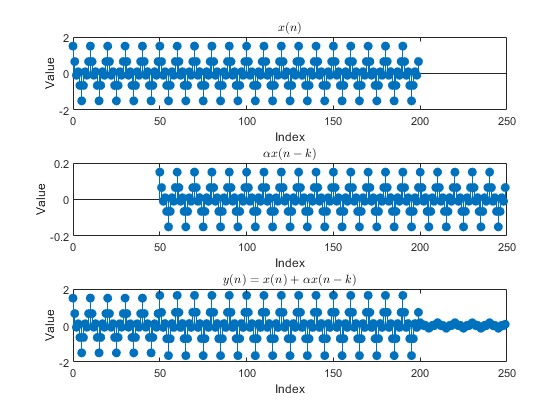
\includegraphics[width=0.9\textwidth]{HW2_13}
    \caption{P2.10.2}
    \label{P2.10.2}
\end{figure}

\addcontentsline{toc}{section}{P2.11}
\section*{P2.11}

\subsection*{System 1}
\begin{gather*}
    T[x(n)] = x(n)u(n)\\
    aT[x(n)] + bT[y(n)]=ax(n)u(n) + by(n)u(n)\\
    T[ax(n) + by(n)] = (ax(n) + by(n))u(n)
    = ax(n)u(n) + by(n)u(n)\\
    ax(n)u(n) + by(n)u(n) \overset{?}{=} ax(n)u(n) + by(n)u(n)
\end{gather*} The above equality is satisfied; thus, System 1
is indeed linear.

\subsection*{System 2}
\begin{gather*}
    T[x(n)] = x(n) + nx(n+1)\\
    aT[x(n)] + bT[y(n)] = ax(n) + anx(n+1) + by(n) + bny(n+1)\\
    T[ax(n) + by(n)] = ax(n) + by(n) + n(ax(n+1) + by(n+1))
    \\= ax(n) + by(n) + anx(n+1) + bny(n+1)\\
    ax(n) + by(n) + anx(n+1) + bny(n+1) \\ \overset{?}{=}
    ax(n) + anx(n+1) + by(n) + bny(n+1)
\end{gather*} The above equality is satisfied; thus, System 2
is indeed linear.

\subsection*{System 3}
\begin{gather*}
    T[x(n)] = x(n) + \frac12 x(n-2) - \frac13 x(n-3)x(2n)\\
    aT[x(n)] + bT[y(n)] = ax(n) + \frac{a}2 x(n-2) - \frac{a}3 x(n-3)x(2n)\\+ by(n) + \frac{b}2 y(n-2) - \frac{b}3 y(n-3)y(2n)\\
    T[ax(n) + by(n)] \\= ax(n) + by(n)
    +\frac12(ax(n-2) + by(n-2))
    \\-frac13(ax(n-3) + by(n-3))(ax(2n) + by(2n))
\end{gather*} I can stop here, because as you can see on the
last line, I am going to get \(a^2\), which is not present in
\(aT[x(n)] + bT[y(n)]\). Therefore, System 3 is not linear.

\subsection*{System 4}
\begin{gather*}
    T[x(n)] = \sum_{k = -\infty}^{n+5} 2x(k)\\
    aT[x(n)] + bT[y(n)] = 2a\sum_{k = -\infty}^{n+5} x(k) + 2b\sum_{k = -\infty}^{n+5} y(k)\\
    T[ax(n) + by(n)] = 2\sum_{k = -\infty}^{n+5} (ax(k) + by(k))\\
    = 2a\sum_{k = -\infty}^{n+5} x(k) + 2b\sum_{k = -\infty}^{n+5} y(k)\\
    aT[x(n)] + bT[y(n)] \overset{?}{=} T[ax(n) + by(n)]
\end{gather*}The above equality is satisfied; thus, System 4
is indeed linear.

\subsection*{System 5}
\begin{gather*}
    T[x(n)] = x(2n)\\
    aT[x(n)] + bT[y(n)] = ax(2n) + by(2n)\\
    T[ax(n) + by(n)] = ax(2n) + by(2n)\\
    aT[x(n)] + bT[y(n)] \overset{?}{=} T[ax(n) + by(n)]
\end{gather*}The above equality is satisfied; thus, System 5
is indeed linear.

\subsection*{System 6}
\begin{gather*}
    T[x(n)] = \operatorname{round}(x(n))\\
    aT[x(n)] + bT[y(n)] = a\operatorname{round}(x(n)) + b\operatorname{round}(y(n))\\
    T[ax(n) + by(n)] = \operatorname{round}(ax(n) + by(n))\\
    aT[x(n)] + bT[y(n)] \overset{?}{=} T[ax(n) + by(n)]
\end{gather*} The above equality is not satisfied;
thus, System 6 is not linear.

\subsection*{System 7}
\begin{gather*}
    T[x(n)] = x(-n)\\
    aT[x(n)] + bT[y(n)] = ax(-n) + by(-n)\\
    T[ax(n) + by(n)] = ax(-n) + by(-n)\\
    aT[x(n)] + bT[y(n)] \overset{?}{=} T[ax(n) + by(n)]
\end{gather*} Yes this is linear.
\begin{gather*}
    T[x(n - k)] = x(-n - k)\\
    y(n-k) = x(-(n-k)) = x(-n+k)
\end{gather*} Time variant.

\begin{figure}[htbp]
    \centering
    
    \caption{<caption>}
    \label{<label>}
\end{figure}

\end{document}
